% Chapter 1

\chapter{Introduction}\label{ch:introduction} % For referencing the chapter elsewhere, use \autoref{ch:introduction} 


The Internet can be defined as  \emph{a global system of interconnected computer networks}, and  since the appearance of the World Wide Web (WWW) in 1989, it has been constantly changing and growing, becoming a vital part of our lives in  contemporary society \cite{Morris1996}.  Before the ubiquitous presence of the Internet and the WWW,  people had access to books only in libraries, films in cinemas or rental shops, and records were sold in physical format. Thus,  access was limited and difficult. As physical storage was needed, it was impossible to find every book (film or record) in the same physical space at once. Nowadays the access problem is solved, and people have access to these and many other products and services through smart devices connected to the Internet. However, the solution of the information access problem led to an information overload problem. For example, in the 80's a common user had access to hundreds of songs, while nowadays streaming services like Spotify\footnote{\url{http://www.spotify.com}} provide access to dozens of millions of songs.  Moreover, traditional ways of content discovery such as the so-called \emph{word of mouth} on physical social networks (neighbours, family or friends) have been translated into their online counterparts (Facebook\footnote{\url{http://facebook.com}}, Twitter\footnote{\url{http://twitter.com}}, etc.), changing the way content is discovered and consumed. 

As access to media becomes easier, and the amount of user generated content builds up, there is an increasing difficulty when dealing with the vast amount of information which is available. Finding a new movie to watch, discovering new bands to listen to, or deciding whom to follow in an online social network is becoming increasingly difficult for the user. In fact, we often find ourselves overloaded with information and choice. Therefore, there is a need for a new class of  intelligent systems that help us to navigate through all this information, by automatically identifying  relevant content and filtering  that which is irrelevant. Recommender systems \cite{Aman2010, Ricci2011, Levy2010a, Resnick1997, Schafer1999} perform this task by learning the products and services we like, the news articles we find interesting, or the music we listen to. All this knowledge is then applied to personalise the user experience in different services; from advertising to clothes recommender systems, from movie recommender systems to music discovery. Thus, much of the content that users access on the internet can be filtered according to their needs in a personalised fashion. 


Recommender systems are a class of information filtering systems which aim to present information in a personalised fashion, aiding the user to browse large collection of items, i.e., scientific articles \cite{Toscher2009} or movies  \cite{Wang2011, Golbeck2006} . These type of  systems have been widely exploited in the last decade, and are often found on internet sites dealing with large amounts of information such as Netflix\footnote{\url{http://www.netflix.com}} (video streaming platform) or Spotify (music streaming platform). Moreover, the concept of recommender system is very broad. For example, they have been used in collaborative search using reputation systems \cite{Mahony2010},  to get recommendations of people to follow in social networks \cite{Hannon2010}, to classify news feeds \cite{Phelan2012, Esparza2013} or to help users navigate through large collections of products reviews in an e-commerce scenario \cite{Dong2012}, among many other applications.


Figure \ref{fig:netflix1} shows the Netflix web interface,  which is completely personalised. For example, the movies in the \emph{top picks} row are shown based on the user's past behaviour, while the second row shows similar items to a previously watched (and liked) television show.


\begin{figure}[h!] 
  \centering
    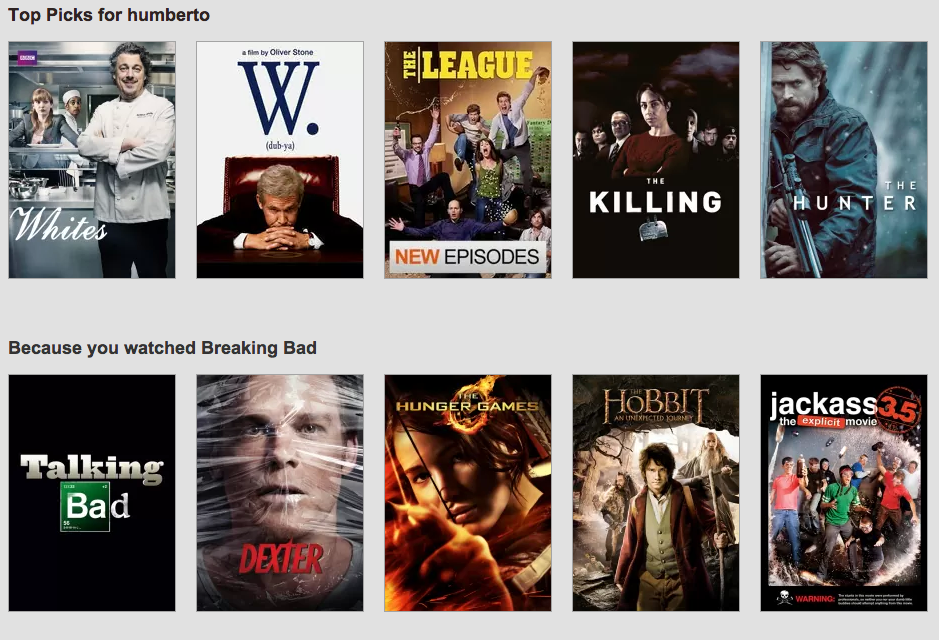
\includegraphics[width=1\textwidth]{figures/netflix.png}
  \caption{The Netflix user interface shows different recommendations streams.}
   \label{fig:netflix1}
\end{figure}

Figure \ref{fig:amazon1} shows the non-personalised recommendations generated by the popular e-commerce site Amazon\footnote{ \url{http://www.amazon.com}}, based on the "people who bought this also bought that" model of recommendation, not taking in account the user's previous interaction with the system.


\begin{figure}[h!] 
  \centering
    
\includegraphics[width=1\textwidth]{figures/amazon1}
  \caption{Amazon present users with non-personalised recommendations of similar items calculated by shopping co-ocurrence.}
   \label{fig:amazon1}
\end{figure}


Recommender systems can be classified according to the information they use when generating recommendations. \emph{Collaborative recommender systems (CF)} \cite{Sarwara, Koren2008, Bell2007} use the wisdom of the crowd to identify trends on how users interact with the system. They are able to find like-minded users and use that information to make recommendations, relying only on preference data from the users in the system. These type of algorithms are widely present in commercial systems such as the e-commerce platform Amazon \cite{Linden2003}, which uses item-to-item collaborative recommendations. Moreover, they have proven to be accurate, specially thanks to advances developed in the context of the Netflix Prize \cite{Bennett2007}. \emph{Content-based Filtering (CBF) recommender systems} \cite{Meteren, Lops2011,  Pazzani2007}  utilise user feedback provided by users to generate recommendations of similar items to those users have liked in the past, by analysing the content metadata. These type of systems are particularly useful in cases where the access to other user's preferences is limited but rich metadata is available, for example in the case of television recommendations \cite{Blanco-Fernandez2008}. \emph{Hybrid systems} \cite{Modeling2002, Bostandjiev2012} usually combine content-based with collaborative filtering approaches, with the aim of obtaining a better performance than with a single approach, while reducing the drawbacks of each approach. The most commonly used hybrid approaches are \emph{weighted hybrid recommenders}, \emph{switching hybrid recommenders} and \emph{mixed hybrid recommenders}, as described in \cite{Modeling2002}.

An interesting and widely studied area of recommender systems is evaluation \cite{Herlocker2004, Shani}. Traditionally, recommender systems evaluation focused on measuring accuracy. However, in recent times the focus has extended to measure recommender systems properties  beyond accuracy \cite{Konstan2012, McNee2006a} such as diversity, popularity, novelty or serendipity. Performing an evaluation that considers all these facets is necessary to better understand all the factors that affect the performance of this type of systems and how they affect the enhancement of content discovery. Moreover, there is a growing interest in studying the evaluation of recommender systems considering not only \emph{offline evaluation} experiment, but also \emph{user studies} and \emph{A/B testing} \cite{Shani}.


The music industry has dramatically changed in the last decades and has become an example of a scenario where information overload is a critical problem. The formats and devices in which music is played have changed several times;  from vinyl, to cassettes, CDs, mp3 players and finally to smartphones. Products like the iPod\footnote{\url{https://www.apple.com/ipod/}} (first released in 2001) or services like Napster\footnote{\url{http://ie.napster.com/start}} (a P2P music sharing service first released in 2000) challenged the traditional music distribution channels such as record stores and radios. More recently, services like Last.FM\footnote{\url{http://www.last.fm/}} (which allows users to track and tag all the music listened to), Spotify or  rdio\footnote{\url{http://www.rdio.com/}}  are disrupting the traditional music business model, based in the purchase of albums in physical stores, shifting users towards a monthly payment model with unlimited access to vast music catalogs. In this context, music discovery, classification and recommendation has become a more important part of each of these products, driving  research both in industry and academia \cite{Levy2010a, Celma2011, Aman2010, Celma2009}. 

 \begin{figure}[h!]
\centering
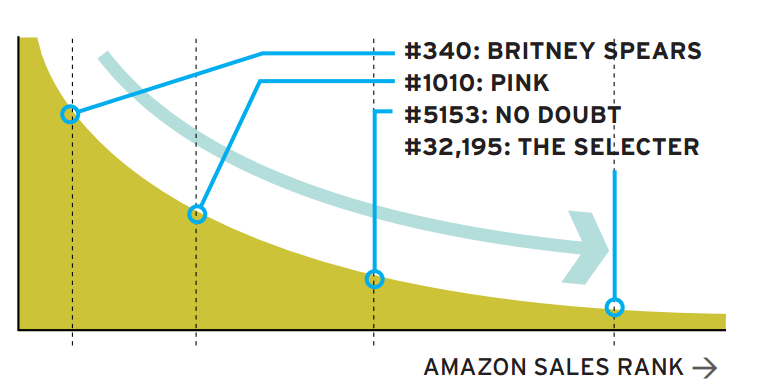
\includegraphics[width=1 \textwidth]{figures/top_amazon}
\caption{Sales per artist on the e-commerce website Amazon.com, from the 2010 Wired Magazine article \emph{The Long Tail}, by Chris Anderson \cite{Anderson2004}.}
\label{fig:top_mine}
\end{figure}


Even when effort has been put into enabling music discovery, overall listening behaviour has, however, not changed, and still follows a long tail distribution. Thus, a very reduced amount of artists are extremely popular, while there is a  long list of artists and songs that rarely get sold or listened to. An example is pictured in Figure \ref{fig:top_mine}, which shows total sales per artist on the e-commerce site Amazon (vertical axis) sorted by popularity (horizontal axis). Here, the total number of records sold by artists like \emph{Britney Spears} are several orders of magnitude bigger than other less popular artists such as \emph{The Selecter}. Thus, the long tail of artists needs to be exploited when generating recommendations to increase sales, artist visibility, and provide novel recommendations to the consumer.

 
The problem of music discovery has been widely studied in recent times and several reviews of the field have been published \cite{Song2012, Celma2009, Celma2011}.  One of the approaches to solve the information overload in this field is by automatically classifying music, which allows sorting large music collections or automatically generating playlist and recommendations. This type of approach has been successfully used to generate music recommendations based on mood  \cite{Han2009} and genre \cite{Hu2012}. For example, Figure \ref{fig:spotify_recs} shows the Spotify desktop application interface, where playlists are classified according to their moods and genres.

%The classification problem is often divided according to the type of data available in the training process. In \emph{supervised learning} \cite{Mccallum1997, IanH.Witten2005} the classifier uses labeled data to learn a model, and then classifies new instances based on that model. In  \emph{unsupervised learning}  \cite{Cord2001, Barlow1989} (often referred as clustering)  the data is partitioned without using predefined class labels, thus it is the algorithm which decides how to best partition the data into a predefined number of clusters.  


  \begin{figure}[h!]
\centering
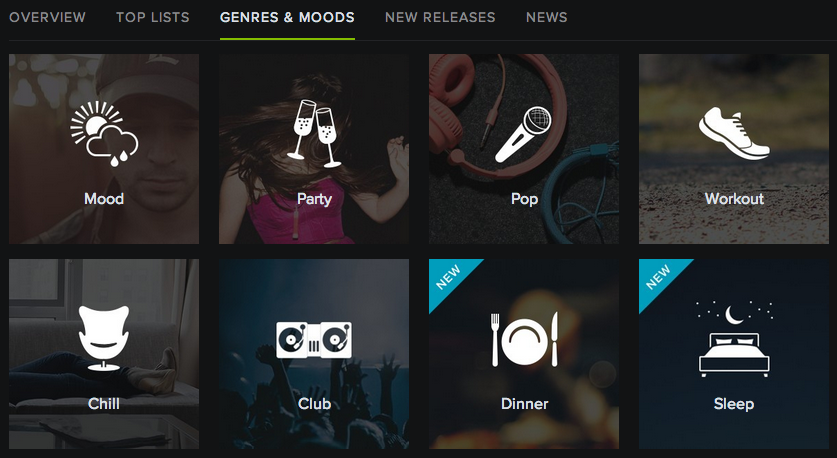
\includegraphics[width=1 \textwidth]{figures/spotify_2}
\caption{The Spotify interface, showing  different mood and genre playlists.}
\label{fig:spotify_recs}
\end{figure}
 


\section{Motivations}

\blindtext


%% FINISHING PARAGRAPH

\section{Contributions}

\blindtext



\section{Thesis Overview}

The remainder of this thesis is organised in two parts. In the first part we study the general problem of recommender systems evaluation. In the second part we focus on the particular problem of music discovery, from the perspective of music mood and genre classification.


In the first part, Chapter \ref{ch:background} provides an overview of recommender systems, focusing on collaborative filtering algorithms and the different techniques and metrics used for evaluating them. Chapter \ref{ch:evaluation} presents two experiments on collaborative filtering algorithms evaluation. The first is a comprehensive analysis of collaborative filtering algorithms in different scenarios, where the performance of the algorithms is measured in terms of top-N accuracy metrics, and metrics beyond accuracy, such as popularity, diversity, reach or coverage. The second experiment presents a comparative analysis of the two main neighbourhood-based collaborative filtering algorithms. Here, we study how the number of neighbours in the \emph{UKNN} algorithm affects its performance in terms of precision, diversity and popularity.

In the second part of this thesis, Chapter \ref{section:chapter4} deals with the problem of classification. It describes the different algorithms, the vector space model, and presents a discussion on the related work for music mood and genre classification. Chapter \ref{section:chapter5} presents two experiments that evaluate our proposed approach for music mood and genre classification using a supervised classification strategy. We study a classification approach based on  ANEW-derived metafeatures, and we compare the results with the standard vector space model approach, considering also  different term weightings. Moreover, the proposed approaches are evaluated using a large freely-available dataset.


Finally, Chapter \ref{chap:conc} presents the conclusions derived from the work carried out in this thesis. Here, we highlight the key findings from  each of the experiments presented, and several lines of future work related to the thesis are further discussed.

